% some changes 

\documentclass{exam}

\usepackage{fullpage}
\usepackage{enumerate}
\usepackage{siunitx} 
\usepackage{graphicx}
\usepackage[fleqn]{amsmath}
\usepackage{cancel}
\usepackage{polynom}
\usepackage{float}
\usepackage{mdwlist}
\usepackage{booktabs}
\usepackage{cancel}
\usepackage{polynom}
\usepackage{caption}

\newcommand{\degree}{\ensuremath{^\circ}} 
\everymath{\displaystyle}

% \begin{figure}[H]
%   \centering
%   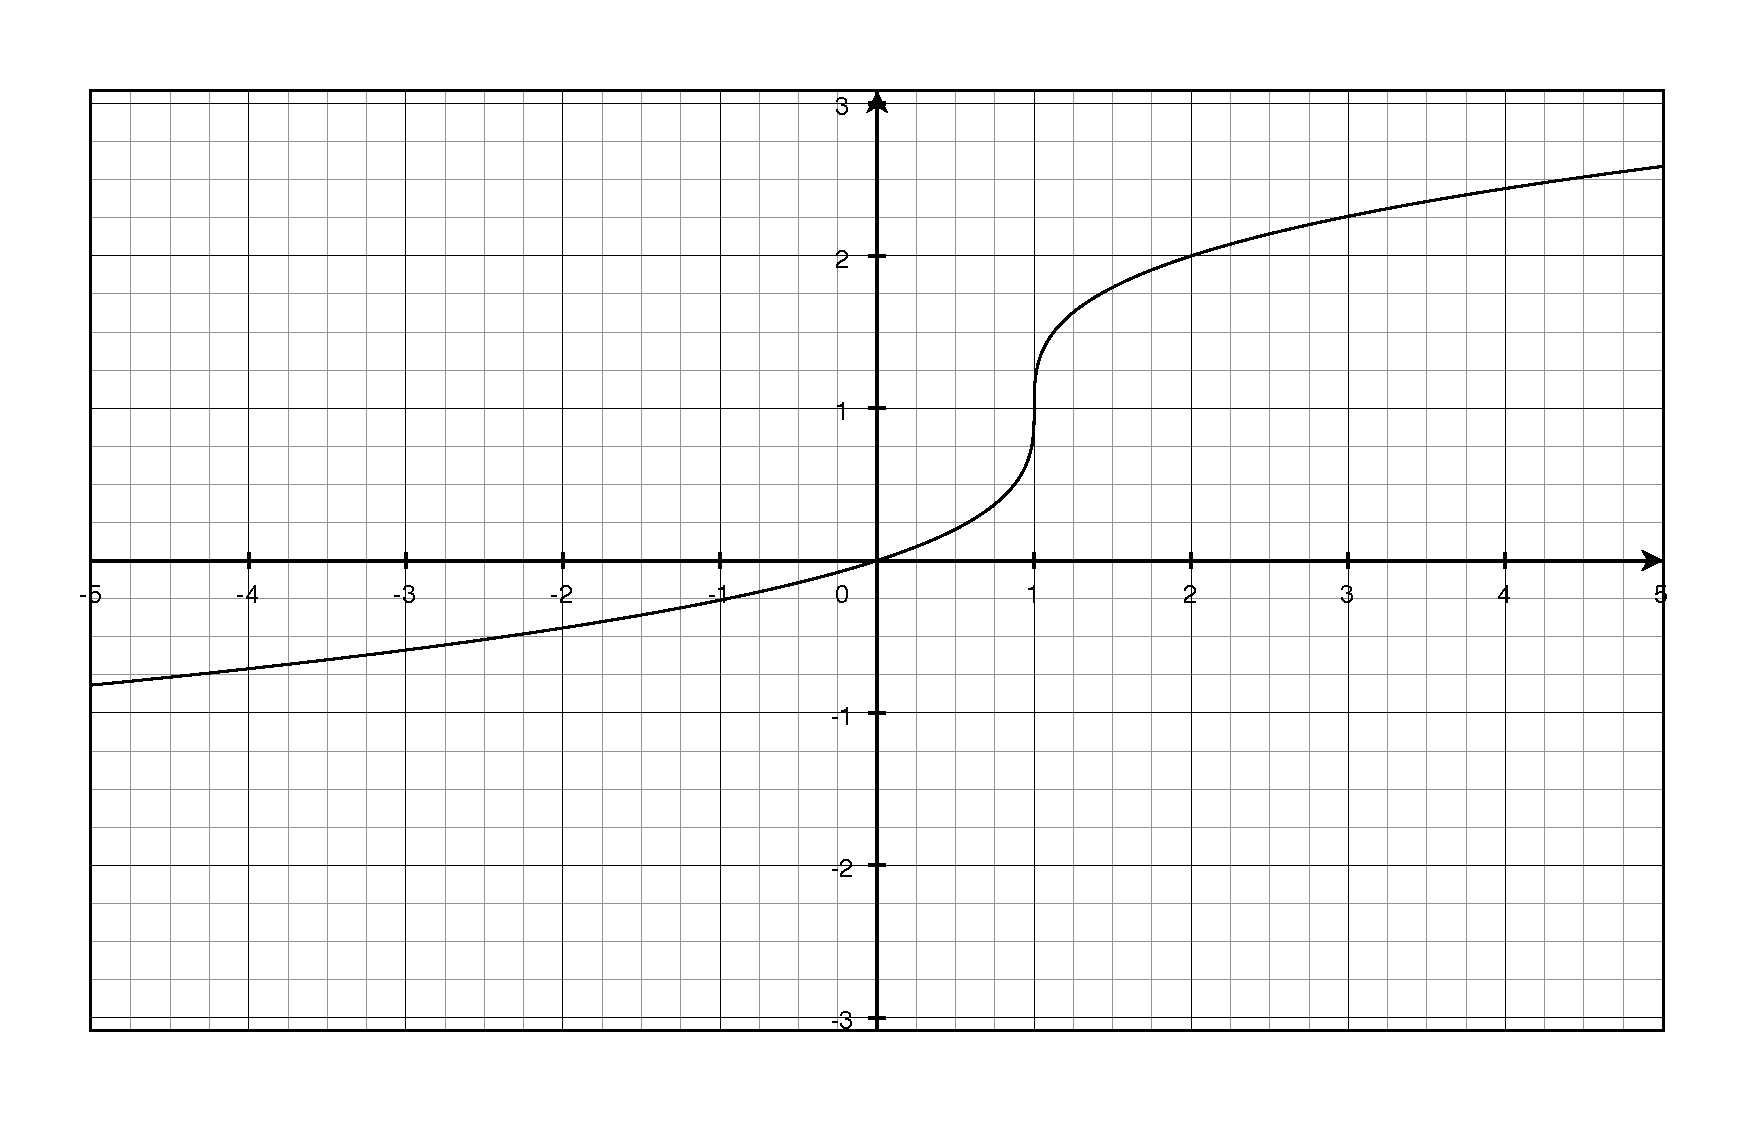
\includegraphics[scale=.3]{question7.eps}
%   \caption*{Question 7}
% \end{figure}

% \begin{tabular}{cc}
% \toprule
% period & amplitude \\
% \midrule
%   $\pi$ & $2$ \\
% \bottomrule
% \end{tabular}

% \textwidth 6.5 in

\printanswers

\ifprintanswers 
\usepackage{2in1, lscape} 
\fi

\title{Math 263a \\ Homework Four}
\date{February 8, 2012}

\begin{document}

\maketitle

\ifprintanswers
\else
\section{Administrative}
No class next week (2/15), as I'll be out of town.
\fi

\section{Homework}

\begin{itemize*}
  \item Read Section 2.6
  % \item pp 78-79: 2, 7-12
  \item pp 78-79: 14, 16-18
  \item pp 84-86: 5-8, 15-22, 25-26, 29-30, 41-44
\end{itemize*}

\section{Extra Credit}


Use the {\em Squeeze Theorem} to prove that 
\[
  \lim_{x \to 0} |x| \sin^2 \frac{1}{x} = 0
\]

\begin{solution}

Since $-1 \leq \sin \theta \leq 1$ for any value of $\theta$, $0 \leq \sin^2 \frac{1}{x} \leq 1$ for any $x$, excluding
0 which is not in the domain.

$|x| \geq 0$, for any $x$.

So $0 \leq |x| \sin^2 \frac{1}{x} \leq |x|$ since the values in the middle are just $|x|$ scaled by a value less than one.

If we let: $f(x) = 0$, $g(x) = |x| \sin^2 \frac{1}{x}$, and $h(x) = |x|$:
\begin{align*}
  \lim_{x \to 0} f(x) &= \lim_{x \to 0} 0 = 0 \\
  \lim_{x \to 0} h(x) &=  \lim_{x \to 0} |x| = 0 \\
\end{align*}
\[
  f(x) \leq g(x) \leq h(x) \text{ for any x} \\
\]

So: $\lim_{x \to 0} g(x) = 0$

\vspace{0.2 cm}

The graph of this function is interesting:

\begin{figure}[H]
  \centering
  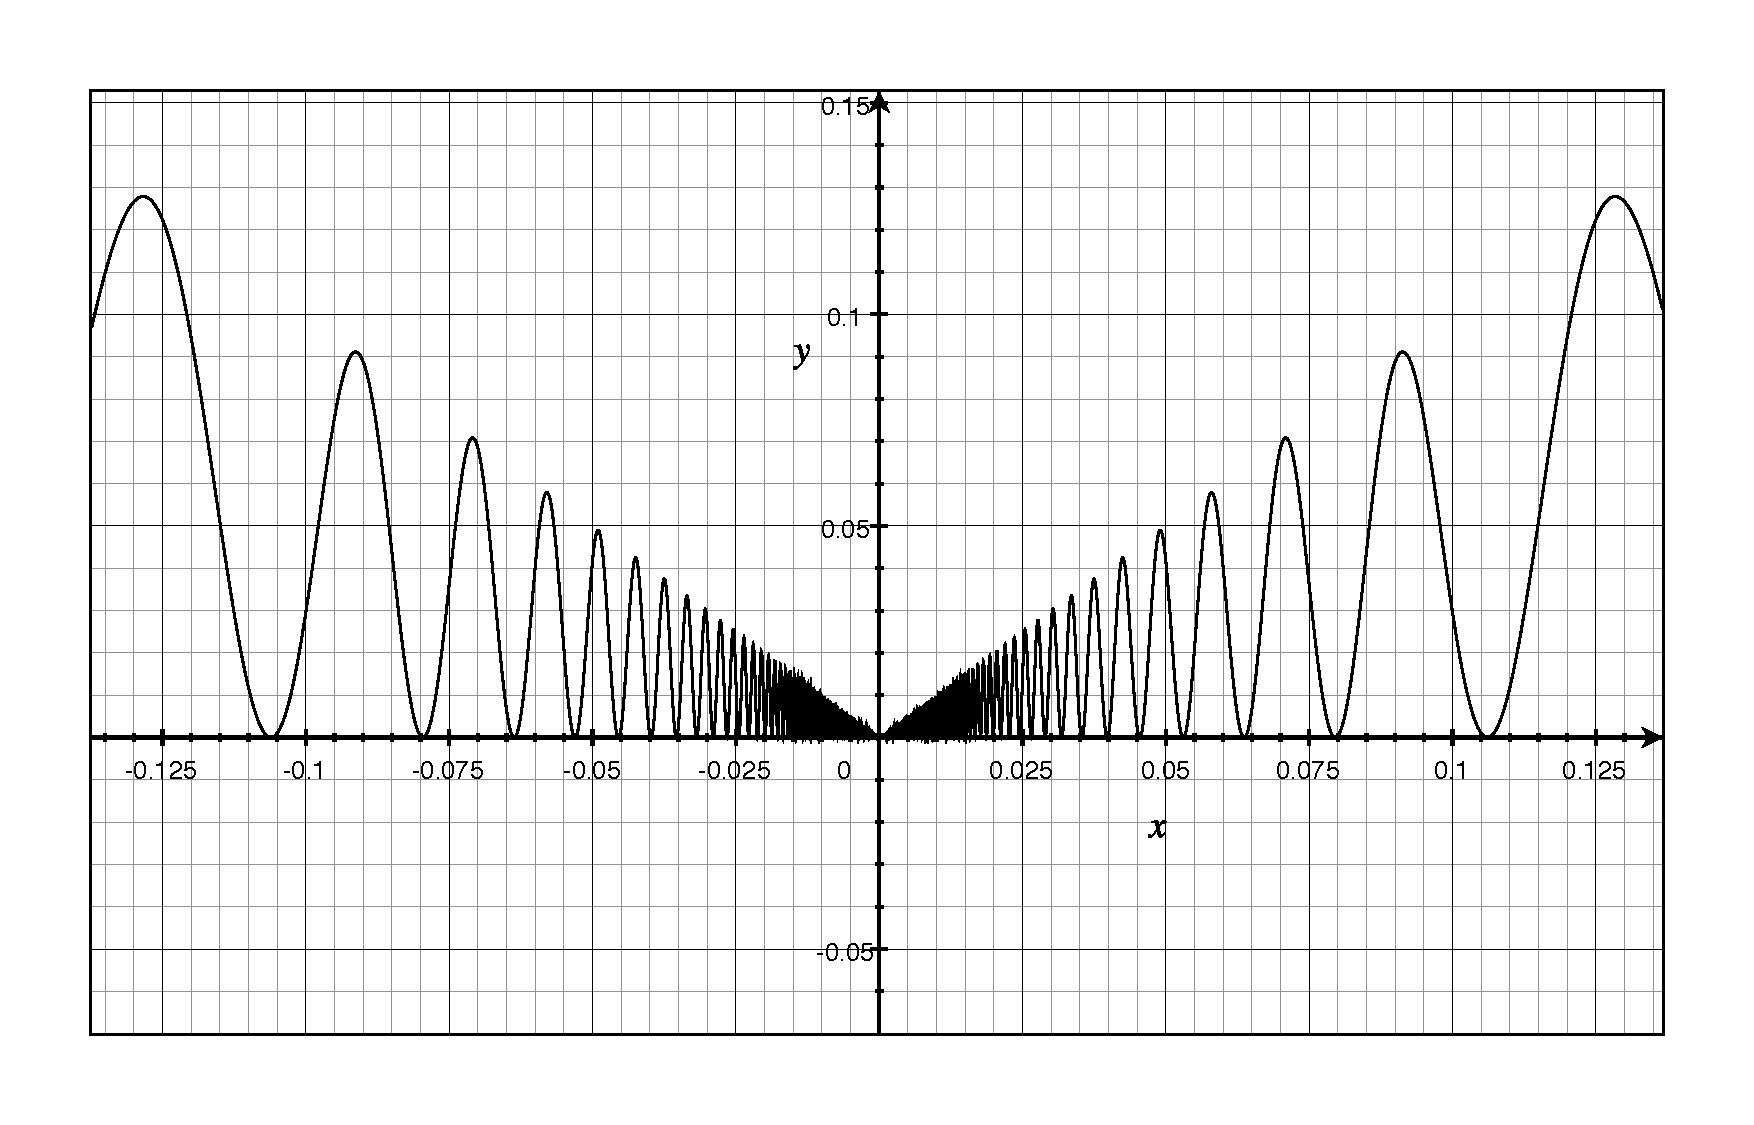
\includegraphics[scale=.3]{extra_credit.eps}
  \caption*{Extra Credit Graph}
\end{figure}

\end{solution}

% \begin{itemize*}
% \item pp 78-79: 27 
% \item pp 78: 27
% \end{itemize*}

\ifprintanswers


\section{Section 2.5}
\begin{description}
\item[14]
To prove: for any $\epsilon$ there is a $\delta$ such that:

if $|x - 1| < \delta$ then $|f(x) - 8| < \epsilon$.

Preliminary Investigation:
\begin{align*}
  \left| \frac{14x^2-20x+6}{x-1} - 8 \right| &< \epsilon \\
  \left| \frac{14x^2-20x+6 - 8x + 8}{x-1} \right| &< \epsilon \\
  \left| \frac{14x^2-28x+14}{x-1} \right| &< \epsilon \\
  % \left| \frac{14(x^2-2x+1)}{x-1} \right| &< \epsilon \\
  \left| \frac{14(x-1)^2}{x-1} \right| &< \epsilon \\
  14 | x-1 | &< \epsilon \\
  | x-1 | &< \frac{\epsilon}{14} \\
\end{align*}

Select $\delta = \frac{\epsilon}{14}$ and show that if $|x| < \delta$ then $|f(x) - 8| < \epsilon$:
\[
  \left| \frac{14x^2-20x+6}{x-1} - 8 \right| =  14 |x-1| < 14 \delta = 14 \left( \frac{\epsilon}{14} \right) = \epsilon
\]

Therefore, if $|x| < \delta$ then $|f(x) - 8| < \epsilon$ when $\delta = \frac{\epsilon}{14}$.

\item[16]
To prove: for any $\epsilon$ there is a $\delta$ such that:

if $|x - 1| < \delta$ then $|f(x) - 3| < \epsilon$.

Preliminary Investigation:
\begin{align*}
  |2x^2 + 1 - 3| &< \epsilon \\
  |2x^2 -2| &< \epsilon \\
  2|x^2 -1| &< \epsilon \\
  2|(x+1)(x-1)| &< \epsilon \\
\end{align*}

The $x+1$ term is problematic, but we can limit its size by keeping $\delta < 1$:
\begin{align*}
  0 &\leq x \leq 2 \\
  1 &\leq x + 1 \leq 3 \\
  & |x+1| \leq 3 \\
\end{align*}

Select $\delta = \min \left\{1, \frac{\epsilon}{6} \right\}$ and show that if $|x| < \delta$ then $|f(x) - 3| < \epsilon$:
\[
  |2x^2 + 1 - 3 | = 2|(x+1)(x-1)| \leq 6 | x-1 | < 6 \delta \leq 6 \left( \frac{\epsilon}{6} \right) = \epsilon
\]

Therefore, if $|x| < \delta$ then $|f(x) - 3| < \epsilon$ when $\delta = \min \left\{1, \frac{\epsilon}{6} \right\}$.

\item[17]
To prove: for any $\epsilon$ there is a $\delta$ such that:

if $|x + 1| < \delta$ then $|f(x) - 2| < \epsilon$.

Preliminary Investigation:
\begin{align*}
  |x^2 - 2x - 1 -2| &< \epsilon \\
  |x^2 - 2x - 3| &< \epsilon \\
  |(x-3)(x+1)| &< \epsilon \\
\end{align*}

The $x-3$ term is problematic, but we can limit its size by keeping $\delta < 1$:
\begin{align*}
  -2 &\leq x \leq 0 \\
  -5 &\leq x - 3 \leq -3 \\
  & |x-3| \leq 5 \\
\end{align*}

Select $\delta = \min \left\{1, \frac{\epsilon}{5} \right\}$ and show that if $|x| < \delta$ then $|f(x) - 2| < \epsilon$:
\[
  |x^2 -2x - 1 - 2 | = |(x+1)(x-3)| \leq 5 | x+1 | < 5 \delta \leq 5 \left( \frac{\epsilon}{5} \right) = \epsilon
\]

Therefore, if $|x| < \delta$ then $|f(x) - 2| < \epsilon$ when $\delta = \min \left\{1, \frac{\epsilon}{5} \right\}$.

\item[18]
To prove: for any $\epsilon$ there is a $\delta$ such that:

if $|x| < \delta$ then $|x^4| < \epsilon$.

Preliminary Investigation:
\begin{align*}
  |x^4| &< \epsilon \\
  |x|^4 &< \epsilon \\
  |x| &\leq \sqrt[4]{\epsilon}
\end{align*}

Select $\delta = \sqrt[4]{\epsilon}$ and show that if $|x| < \delta$ then $|x^4| < \epsilon$:
\[
  |x^4| = |x|^4 < \delta^4 = (\sqrt[4]{\epsilon})^4 = \epsilon
\]

Therefore, if $|x| < \delta$ then $|x^4| < \epsilon$ when $\delta = \sqrt[4]{\epsilon}$.

\end{description}

\section{Section 2.6}
\begin{description}

\item[5]
\begin{align*}
  \lim_{x \to 2} \frac{2x + 1}{5 - 3x} &= \frac{\lim\limits_{x \to 2} 2x + \lim\limits_{x \to 2} 1}{\lim\limits_{x \to 2} 5 - \lim\limits_{x \to 2} 3x} \\
  &= \frac{2 \lim\limits_{x \to 2} x + 1}{5 - 3 \lim\limits_{x \to 2} x} \\
  &= \frac{2 \cdot 2 + 1}{5 - 3 \cdot 2} \\
  &= -5 \\
\end{align*}

\item[6]
\begin{align*}
  \lim_{x \to -3} \frac{4x^3 + 1}{7-2x^2} &= \frac{\lim\limits_{x \to -3} 4x^3 + 1}{7- \lim\limits_{x \to -3} 2x^2} \\
   &= \frac{4 \lim\limits_{x \to -3} x^3 + 1}{7- 2 \lim\limits_{x \to -3} x^2} \\
   &= \frac{4 \left( \lim\limits_{x \to -3} x \right) ^3 + 1}{7- 2 \left( \lim\limits_{x \to -3} x \right)^2} \\
   &= \frac{4 (-3)^3 + 1}{7- 2 (-3)^2} \\
   &= \frac{107}{11} \\
\end{align*}

\item[7]
\begin{align*}
  \lim_{x \to 3} \sqrt{3x - 5} &= \sqrt{\lim_{x \to 3} 3x - 5} \\
  &= \sqrt{3 \lim_{x \to 3} x - 5} \\
  &= \sqrt{3 \cdot 3 - 5} \\
  &= \sqrt{4} \\
  &= 2 \\
\end{align*}

\item[8]
\begin{align*}
  \lim_{x \to -3} \sqrt{5x^2 + 2x} &= \sqrt{\lim_{x \to -3} 5x^2 + \lim_{x \to -3} 2x} \\
   &= \sqrt{5 \lim_{x \to -3} x^2 + 2 \lim_{x \to -3} x} \\
   &= \sqrt{5 \left( \lim_{x \to -3} x \right)^2 + 2 (-3)} \\
   &= \sqrt{5 (-3)^2 + 2 (-3)} \\
   &= \sqrt{39} \\
\end{align*}

\item[15]
\begin{align*}
  \lim_{x \to -1} \frac{x^2 + x - 2}{x^2 - 1} &= \lim_{x \to -1} \frac{(x+2)(x-1)}{(x+1)(x-1)} \\
    &= \lim_{x \to -1} \frac{x+2}{x+1} \\
\end{align*}

The limit does not exist since the denominator approaches 0 as $x$ approaches -1.

\item[16]
\begin{align*}
  \lim_{x \to 2} \frac{x^2 + 7x + 10}{x+2} &= \lim_{x \to 2} \frac{(x+5)(x+2)}{x+2} \\
   &= \lim_{x \to 2} x+5 \\
   &= 7 \\
\end{align*}

\item[17]
\begin{align*}
  \lim_{x \to 1} \frac{x^2 + x - 2}{x^2 - 1} &= \lim_{x \to 1} \frac{(x+2)(x-1)}{(x+1)(x-1)} \\
   &= \lim_{x \to 1} \frac{x+2}{x+1} \\
   &= \frac{1+2}{1+1} \\
   &= \frac{3}{2} \\
\end{align*}

\item[18]
\begin{align*}
  \lim_{x \to -3} \frac{x^2 - 14x - 51}{x^2 - 4x - 21} &= \lim_{x \to -3} \frac{(x-17)(x+3)}{(x-7)(x+3)} \\
   &= \lim_{x \to -3} \frac{x-17}{x-7} \\
   &=  \frac{-3-17}{-3 - 7} \\
   &= 2 \\
\end{align*}

\item[19]
\begin{align*}
  \lim_{u \to -2} \frac{u^2 - ux + 2u - 2x}{u^2 - u - 6} &= \lim_{u \to -2} \frac{u(u - x) + 2(u - x)}{(u-3)(u+2)} \\
   &= \lim_{u \to -2} \frac{(u+2)(u - x)}{(u-3)(u+2)} \\
   &= \lim_{u \to -2} \frac{u - x}{u-3} \\
   &= \frac{-2 - x}{-2-3} \\
   &= \frac{x + 2}{5} \\
\end{align*}

\item[20]
\begin{align*}
  \lim_{x \to 1} \frac{x^2 + ux - x - u}{x^2 + 2x - 3} &= \lim_{x \to 1} \frac{x(x + u) - (x + u)}{(x+3)(x-1)} \\
   &= \lim_{x \to 1} \frac{(x-1)(x + u)}{(x+3)(x-1)} \\
   &= \lim_{x \to 1} \frac{x + u}{x+3} \\
   &= \lim_{x \to 1} \frac{u + 1}{4} \\
\end{align*}

\item[21]
\begin{align*}
  \lim_{x \to \pi} \frac{2x^2 - 6x\pi + 4\pi^2}{x^2 - \pi^2} &= \lim_{x \to \pi} \frac{2(x - \pi)(x - 2\pi)}{(x+\pi)(x - \pi)} \\
   &= \lim_{x \to \pi} \frac{2(x - 2\pi)}{x+\pi} \\
   &= \frac{2(\pi - 2\pi)}{\pi+\pi} \\
   % &= \frac{-2\pi}{2 \pi} \\
   &= -1 \\
\end{align*}

\item[22]
\begin{align*}
  \lim_{w \to -2} \frac{(w+2)(w^2 - w - 6)}{w^2 + 4w + 4} &= \lim_{w \to -2} \frac{(w+2)(w-3)(w+2)}{(w+2)^2} \\
   &= \lim_{w \to -2} w-3 \\
   &= -5 \\
\end{align*}

\item[25]
\begin{align*}
  \lim_{x \to a} \sqrt[3]{g(x)} \cdot [f(x) + 3] &= \sqrt[3]{\lim_{x \to a} g(x)} \cdot \left[\lim_{x \to a} f(x) + 3 \right] \\
   &= \sqrt[3]{-1} \cdot [3 + 3] \\
   &= -6 \\
\end{align*}

\item[26]
\begin{align*}
  \lim_{x \to a} \left[ f(x) - 3\right]^4 &= \left[ \lim_{x \to a} f(x) - 3\right]^4 \\
   &= \left[3 - 3\right]^4 \\
   &= 0 \\
\end{align*}

\item[29]
\[
  f(2) = 3 \cdot 2^2 = 12
\]

\begin{align*}
  \lim_{x \to 2} \frac{3x^2 - 12}{x-2} &= \lim_{x \to 2} \frac{3(x+2)(x-2)}{x-2} \\
  &= \lim_{x \to 2} 3(x + 2) \\
  &= 12 \\
\end{align*}

\item[30]
\[
  f(2) = 3 \cdot 2^2 + 2 \cdot 2 + 1 = 17
\]

\begin{align*}
  \lim_{x \to 2} \frac{3x^2 + 2x + 1 - 17}{x-2} &= \lim_{x \to 2} \frac{3x^2 + 2x - 16}{x-2} \\
  &= \lim_{x \to 2} \frac{(3x+8)(x-2)}{x-2} \\
  &= \lim_{x \to 2} 3x+8 \\
  &= 14 \\
\end{align*}

\item[41]
\[
  \lim_{x \to -3^+} \frac{\sqrt{3 + x}}{x} = \frac{\sqrt{3 - 3}}{-3} = 0
\]

\item[42]
\[
  \lim_{x \to -\pi^+} \frac{\sqrt{\pi^3 + x^3}}{x} = \frac{\sqrt{\pi^3 + (-\pi)^3}}{-\pi} = 0
\]

\item[43]
\begin{align*}
  \lim_{x \to 3^+} \frac{x-3}{\sqrt{x^2 - 9}} &= \lim_{x \to 3^+} \frac{(x-3)\sqrt{x^2 - 9}}{x^2 - 9} \\
   &= \lim_{x \to 3^+} \frac{(x-3)\sqrt{x^2 - 9}}{(x+3)(x-3)} \\
   &= \lim_{x \to 3^+} \frac{\sqrt{x^2 - 9}}{x+3} \\
   &= 0 \\
\end{align*}

\item[44]
\[
  \lim_{x \to 1^-} \frac{\sqrt{1+x}}{4 + 4x} = \frac{\sqrt{2}}{8} \\
\]

\end{description}
\else

\vspace{7 cm}

{\em For all things have been baptized in the well of eternity and are beyond good and evil; and good and evil
  themselves are but intervening shadows and damp depressions and drifting clouds.}

\vspace{.2 cm}

\hspace{1 cm} --Friedrich Nietzsche

\fi

\end{document}

